%Specify the language and programming environment you used for your implementation.
%Building the corresponding relational tables, according to the proposed ER model described in the previous phase %enforcing the different integrity constraints.  
%The deliverables for this stage include the following items:
\begin{itemize} 
\item{Sample small data snippet}
%The SQL tables that represent the ER project model, along with at least 3-5 rows of concrete data per table.

Our data sets are composed of three classes, which include review data, user data, and business data. As we have mentioned in the context above, our recommendation system focuses on Pennsylvania centered business. Eventually, we have 32134 as total number of users, 111542 of reviews, and 4086 of business units. The figure below displays an original sample data structure in each of the classes.

\begin{figure}[h] 
	%\begin{center}
		\advance\rightskip-1cm
		{\scalebox{0.3}{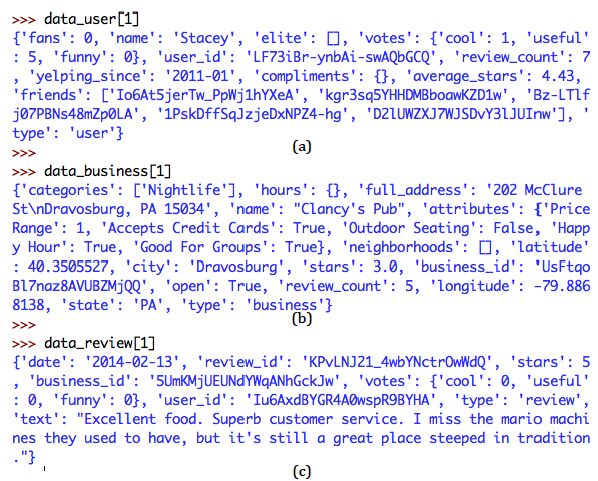
\includegraphics[width=300mm]{sample_data.png}}}
		\caption{Sample data: (a). User Data; (b). Business Data; (c).Review Data}\label{fig:Sample_Data}
	%\end{center}
\end{figure}

\par
We consider a variable significant if it can directly reflex or indirectly help to interpret a user's preference on business units. All the significant variables are then taken into consideration in the recommendation process, with more or less weight. 

For user data, average stars is the average review (level from 0 to 5) a user gave. User id is a unique id code assigned to each user. It is a key variable that relates the three classes of information. And review count, as the total number of review a user has given, will also be used, particularly in the evaluation step. 

For review data, stars indicate how much the reviewer liked this business unit. As star increases, the reviewer likes more. Business id represent each business unit. Finally, user id in review data indicates from who this review was given. 

As for the business data, categories and attributes will be used as characteristic description of a business units through our recommendation system. Business id is a unique code that represents a business store.

\item{Sample small output}
%The normalization steps for each table, along with explanations/justifications of each normalization step.

Given an eligible input user number, the recommendation system generates a recommendation list composed of all business units that has connection to the input user. Each element in the recommendation list has a total score measuring how similar this store is to something the user liked in the past.  Our system chooses business units with greatest score by determining the longest path from the root  node to each third layer nodes. Then it outputs the top ten on which input user has not reviewed before. The result will be an optimal solution based on our item plus user based collaborative filtering algorithm. Below is an example of data output for user 74. 

\begin{figure}[h] 
	\begin{center}
		\advance\rightskip-1cm
		{\scalebox{0.2}{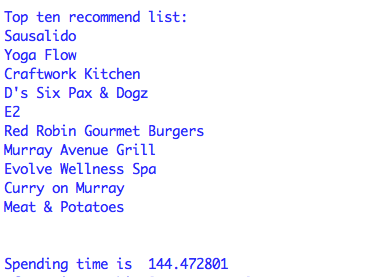
\includegraphics[width=300mm]{sample_output.png}}}
		\caption{Recommendation list for user 74  }\label{fig:Sample_Output}
 \label{fig:top10RecList}
	\end{center}
\end{figure}

\par
As a result, our system is built with relatively hight accuracy and stability. We will show this in following section.
 
\item{Working code}

The code package, as a compressed file with the zip format, is attached in the report. Package includes two zip file named as: maincode.zip and data\_preparation.zip.

\item{Representative of Sample Dataset and Data Size Analysis}
\par
Due to the relatively huge volume of the ``yelp academic dataset", it requires a long processing time for a normal desktop/laptop to execute the data mining task through the whole data set. Thus, only the data from the state of Pennsylvania (labeled as PA in the dataset) are extracted in execution as a sample/demo of our recommendation system. Based the design, our system mainly composes of two sub-procedures: i). generating of clean dataset with specific data structure; ii). Simulating a recommendation list of business units with a given user ID. Here, we provide a space analysis and a demo in the Non-graphical interface.

\par
There are three subsets in the PA data related to business dataset, users dataset and review dataset preserved as the specifically compressed format with sizes of about 5 MB, 19 MB and 111 MB, respectively. All of them are loaded in the RAM. In order to conveniently investigate the required RAM space for the objects during the execution, we utilize the functions in the packages of ``cython" and ``meliae" of Python. These data are separately loaded in the RAM and checked for the required space. The results are shown in Fig. \ref{fig:RAM}. We can see that review dataset requires the maximum RAM space. It is reasonable because the reviews might include some statements with connecting both users and business units. As seen, most of the space are dominated by the unicode strings data (52\%, 47\% and 64\% for the business, user and review dataset, respectively). The total RAM is 555 MB when loading all dataset into RAM with 49 types of variables, which is shown in Fig. \ref{fig:RAM_total}.

\begin{figure}[h] 
	\begin{center}
		\advance\rightskip-1cm
		{\scalebox{0.28}{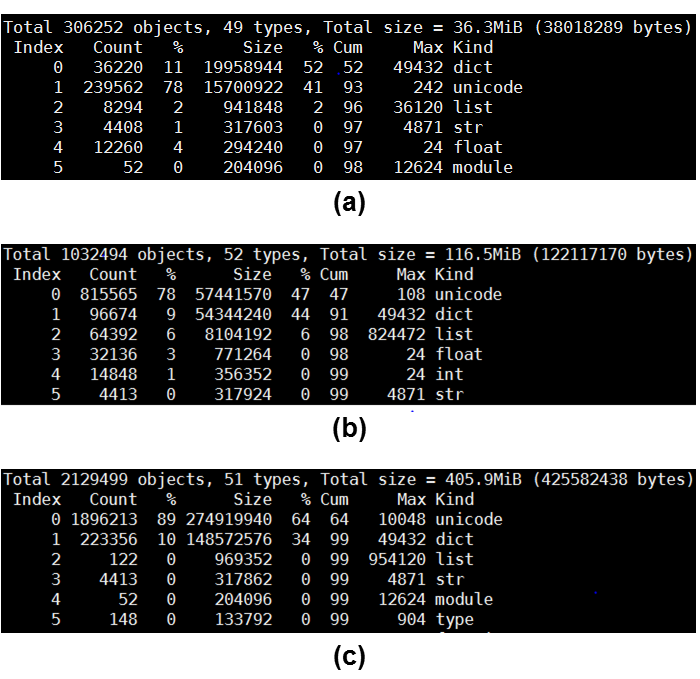
\includegraphics[width=300mm]{RAM.png}}}
		\caption{The require RAM analysis for the input dataset: (a). only business dataset loaded; (b). only user dataset loaded; (c). only review dataset loaded, respectively. The analysis results are from the package of "meliae" in Python.}\label{fig:RAM}
	\end{center}
\end{figure}

\begin{figure}[h] 
	\begin{center}
		\advance\rightskip-1cm
		{\scalebox{0.3}{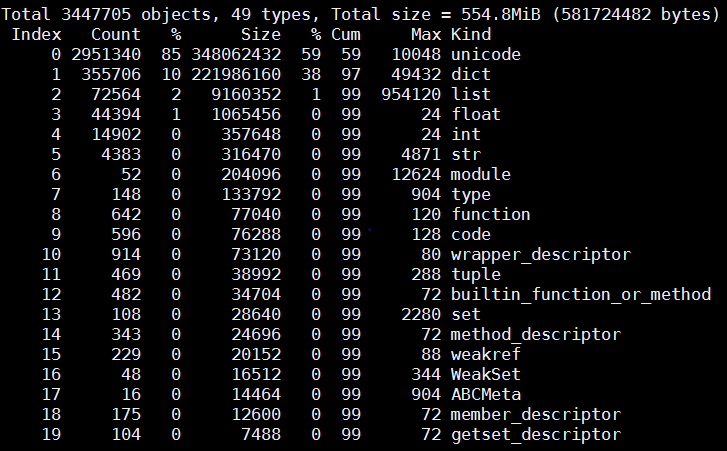
\includegraphics[width=300mm]{RAM_total.png}}}
		\caption{The require RAM analysis for loading the whole representative sample dataset collected from the package of "meliae" in Python.}\label{fig:RAM_total}
	\end{center}
\end{figure}

\item{Sample findings and Demo Result}

As pointed out in the ``Integrity Constraint" subsection, the performance of recommendation system depends on the dataset. In fact, this is one of the basic problem in any task relative to data mining system: valid data is often small. In our system, we can roughly estimate the size of valid data using two rat parameters: the reviews per business unit and the reviews per user. To some extent, we will hope these two ratios are high, which means that there are relationships between the observed users and business units. In our sample data, the reviews per business unit and the reviews per user are 27 and 3. The reviews per business can provides a reference what is a roughly average depth of a recommend graph/tree in our system; in the other hand, the reviews per user can provides a reference about how many new users involved in the next level. To analyze both them in whole dataset might be an extremely complicated task considering that each user has its specific recommendation graph network. Thus, to be simple, we only analyze the distribution of review count per user as shown in Fig. \ref{fig:review_count_per_user}. The distribution is a smooth decreasing curve with the highest point in 1. This means that about 5000 of 32134 users have only a review. As we can see, the curve decrease very fast and the count of users is about 500 when user's review number is at 15. This indicates that only part of users kept writing down their reviews for different business units; this also means that these users have more relationships with others. Our system can provide better recommendation for these users by constructing their graph network with more features. 

\begin{figure}[h] 
	\begin{center}
		\advance\rightskip-1cm
		{\scalebox{0.28}{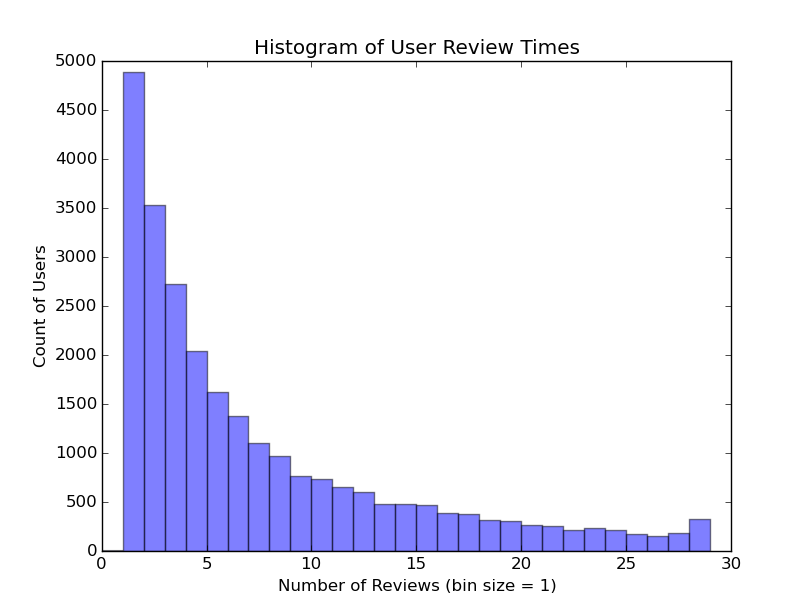
\includegraphics[width=300mm]{review_count_per_user.png}}}
		\caption{Histogram of the reviews for different business units.}\label{fig:review_count_per_user}
	\end{center}
\end{figure}

A demo in the Non-graphical interface is also displayed in Fig. \ref{fig:demo_pipeline}. Here, our system simply accepts the user ID (an integer number) as the input rather than a users' name. Then, a network graph/tree is constructed for the specific input. By following this, our system will extract the existing attributes from the network to look for favorite recommendation with the setting parameters. Finally, a recommendation list including various business units is displayed. This list indicates this user might be interested at looking for the potential consumption from these business units. The performance and execution of our systems strongly depends on the number of existing relationships between the input user and other users. More relationship will induce better performance with fast increasing running time requirement, mainly from the construction of a relationship network.\\ 

\begin{figure}[h] 
	\begin{center}
		\advance\rightskip-1cm
		{\scalebox{0.35}{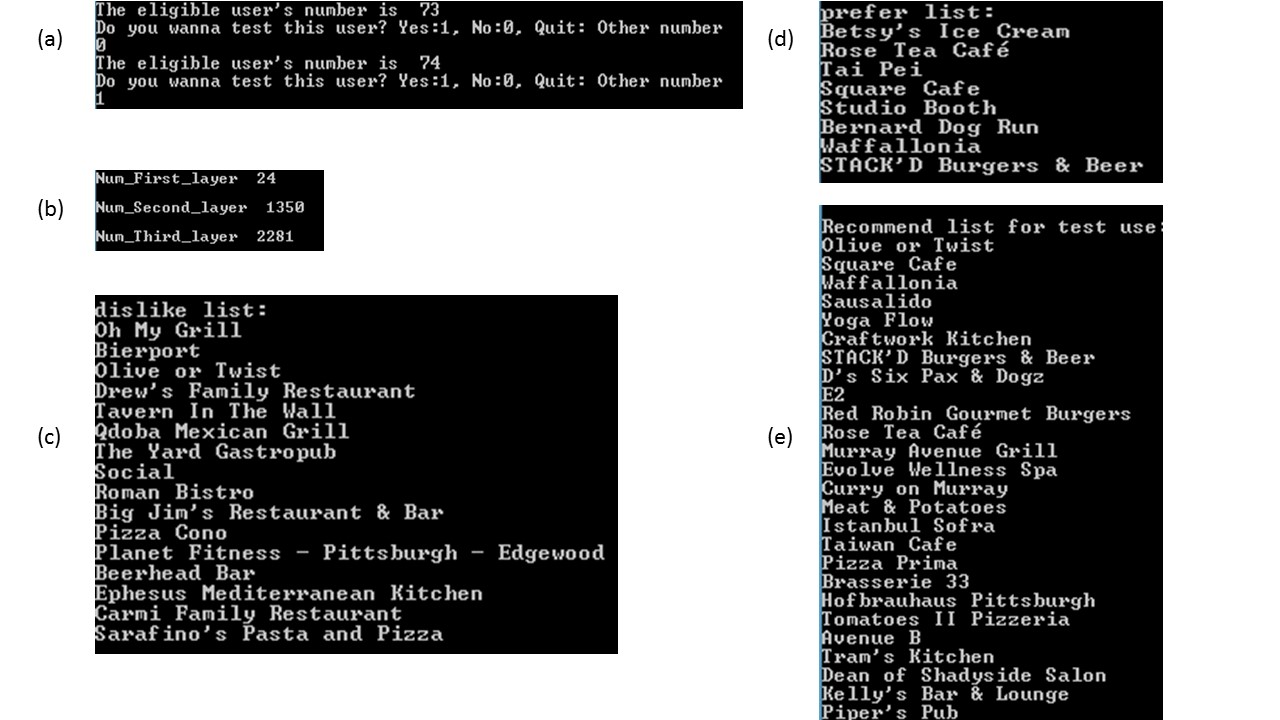
\includegraphics[width=300mm]{demo_pipeline.jpg}}}
		\caption{A demo in the Non-graphical interface: (a) In cmd, using commend "python RecomSys.py" to run the system. A user ID is provided as input. You can execute our recommendation by clicking 1 or skip by clicking 0. Clicking 0 will generate another user ID. Just click any key rather than 0 or 1 to turn off the execution.  (b) The number of nodes (Business Units or Users) in the first three layers are displayed. The first and third layer includes the business units as nodes and the second layer are the users as nodes, who have reviewed the business units in the first layer. (c) A disliked business unit list according to root user in the first layer is also provided. (d) A preferred business unit list according to root user in the first layer is represented. (e) Part of the recommendation list for the test use.(Not the final recommendation list, need remove the business unit that user has already reviewed.)}\label{fig:demo_pipeline}
	\end{center}
\end{figure}

\item{Evaluation on the Algorithm Performance}
\par
It is hard to know if a user is satisfied with our recommendation list, like a example given in Fig. \ref{fig:top10RecList}, without any survey. Thus, we use the following method to evaluate our recommendation system roughly:


Based on existing reviews, we can divide a user's review record into two sets: i). his/her well-liked business units and ii). disliked business units. To evaluate the performance of our recommendation system, we should investigate how well the recommendation list can match in such two set. We will take a pool of size $a$, which is the size of set of well-liked business units, from top of the long recommendation list. We look into the pool, and find out how many business units that the input user reviewed and liked are on list. If there are many such units being re-recommanded, it means the system works well on finding business unit that matched the user's taste. On the contrary, if the pool includes business units that the user reviewed and disliked, we consider it as a poor performance. Then we artifically enlarge the size of pool as 2 $a$, check the performance and stability of the algorithem in this stage.


Because of the time limitation and a bit huge computation, we randomly take 100 eligible users to test the performance of our system and take the average performance.  Table \ref{Tab:eveluate_algorithm} shows the results illustrated by two parameters: Correct Prediction Rate (CPR) and Uncorrect Prediction Rate (UPR). The definitations on CPR and UPR are given in the equations \ref{eqn:PerformanceEqu1} and  \ref{eqn:PerformanceEqu2}.
%%%%%%%%%%%%%%%%%%%%%%%%%%%%%%%%%%%%%%%%%%%%%%%%%%%%%%%%%%%%%% Algorithm Performance
%%%%%%%%%%%%%%%%%%%%%%%%%%%%%%%%%%%%%%%%%%%%%%%%%%%%
\begin{table} 
   \centering

	\caption{Evaluation on the algorithm performance.}
	\begin {tabular}{| p{2.65cm}| p{2.4cm}| p{2.4cm}|} 

	%  \toprule%
	\hline
	 & & \\
	& $|\textnormal{Size of Pool}| = a$ 
	& $|\textnormal{Size of Pool}| = 2a$              \\  [1.4 ex]
	
	\hline	
	 & & \\
	Correction Prediction Rate (CPR)  
	&\hspace{0.8cm}38.1$\%$              
	&\hspace{0.8cm}50.2$\%$  \\  
	[0.6 ex]
	
	\hline	
	 & & \\
	Uncorrection Prediction Rate (UPR)   
	&\hspace{0.8cm}5.4$\%$              
	&\hspace{0.8cm}8.9$\%$  \\ 
	[0.6 ex]
	
	\hline
	\end {tabular}

	\label{Tab:eveluate_algorithm}
\end{table}
%%%%%%%%%%%%%%%%%%%%%%%%%%%%%%%%%

%%%%%%%%%%%%%%%%%%%%%%%%%%%%%%%%%%%%%%%%%%%%%%%%%%%
%%%%%%%  Equation of Performance %%%%%%%%%
%%%%%%%%%%%%%%%%%%%%%%%%%%%%%%%%%%%%%%%%%%%%%%%%%%%

	\begin{align}
	\textnormal{CPR} = \frac{L}{a}  \label{eqn:PerformanceEqu1},\\ 
	\textnormal{UPR} = \frac{D}{b}.
	\label{eqn:PerformanceEqu2}
	\end{align}


where $L$ is the number of business units in the pool correctly recommended by the prediction. This is, they are included in the list of the user's favorite business units. Relatively, $D$ is the number of business units in the pool not matching the user' preference. $a$ is the number of the user's well-liked business units and $b$ is the number of the user's disliked business units in his reviews, respectively.

As shown in Table \ref{Tab:eveluate_algorithm}, the CPR values are 38.1\% and 50.2\% comparing with the UPR values as 5.4\% and 8.9\%, respectively. Obviously, the higher the CPR value, the better the recommendation list. What about the UPR? Our system tries to minimize the UPR value. There are two reasons here. First, if both CPR and UPR are close, it will indicate that our system have weak ability to differentiate a user's favorite business units. In the other, our system also tends to find out user's potentially favorite business units, which have not yet been reviewed by the user. It can be seen as a pure prediction behavior. If the UPR is high, it possibly reveals that these potential business units do not match the user's preference. Based on these viewpoints, our recommendation system has exhibited a considerable and convincing performance. If we double the size of the pool, we observe an increase in both CPR and UPR. Table \ref{Tab:eveluate_algorithm} shows that the CPR increases to 50.2\% from 38.1\%. We found that over half of the preferred business units are in the pool, while the un-preferred business units did not appear very often. UPR stays low as we  increase the size of pool. This results shows that our recommendation system truly detects items that match user's preference. In another word, the disliked items are put in the bottom of the list, while the preferred items are on the top and to be recommended to the user. The result also proves a good stability. Again, the final recommendation list will be the top 10 business units from the long recommendation list that input user has not yet reviewed as shown in Fig.  \ref{fig:top10RecList}.

\end{itemize}



